\chapter{Mapping and Autonomous Navigation}
\label{ch:slam}

\section{Kinect to \gls{slam} Pipeline}
\label{sec:slam_overview}

The system relies on a \textbf{Kinect} depth sensor to generate the environment map.
The extracted depth data is converted into a 2D laser scan. This approach provides the
standard \texttt{sensor\_msgs/LaserScan} message structure expected by the \gls{slam}
algorithm. The \texttt{mapping.launch.py} file launches and orchestrates this entire
chain (Figure~\ref{fig:slam_pipeline}).

\begin{figure}[H]
	\centering
	\resizebox{0.92\linewidth}{!}{%
		\begin{tikzpicture}[
				stage/.style={draw, rounded corners=4pt, minimum height=1.1cm, minimum width=2.7cm,
						fill=EsiGray, font=\scriptsize\bfseries, text=EsiDark, align=center},
				arr/.style={-Stealth, thick, EsiBlue!80},
				lbl/.style={font=\tiny, text=EsiAccent, align=center}
			]
			\node[stage, fill=EsiGreen!15] (kinect) at (0,0) {Kinect (v1)\\\tiny RGB-D sensor};
			\node[stage, fill=EsiGreen!15] (driver) at (3.4,0) {kinect\_ros2\_node\\\tiny libfreenect driver};
			\node[stage, fill=EsiAccent!18] (d2l) at (7.0,0) {depthimage\_to\_\\laserscan\_node};
			\node[stage, fill=EsiBlue!15] (slam) at (10.6,0) {async\_slam\_\\toolbox\_node};
			\node[stage, fill=EsiBlue!15] (rviz) at (10.6,-2.1) {\gls{rviz} 2\\\tiny visualization};

			\draw[arr] (kinect) -- node[lbl, above]{USB} (driver);
			\draw[arr] (driver) -- node[lbl, above]{/kinect/depth/\\image\_raw} (d2l);
			\draw[arr] (d2l) -- node[lbl, above]{/scan\\(LaserScan)} (slam);
			\draw[arr] (slam) -- node[lbl, right]{/map} (rviz);
			\draw[arr] (slam.south) -- ++(0,-0.7) -| node[lbl, pos=0.25, above]{/tf (map$\to$odom)} (rviz.north);
		\end{tikzpicture}
	}
	\caption{Mapping pipeline as orchestrated by \texttt{mapping.launch.py}.}
	\label{fig:slam_pipeline}
\end{figure}

The \texttt{kinect\_ros2} driver (namespace \texttt{kinect}, based on
\texttt{libfreenect}) exposes \topic{/kinect/depth/image\_raw} and
\topic{/kinect/depth/camera\_info}. A \texttt{static\_transform\_publisher} links
\texttt{camera\_depth\_frame} (\gls{urdf}) to the native \texttt{kinect\_depth} frame via
an identity transform. The \texttt{depthimage\_to\_laserscan\_node}
\label{sec:slam_d2l}
node then
projects a horizontal band of the depth image into a synthetic laser scan
(Table~\ref{tab:d2l_params}).

\begin{table}[H]
	\centering
	\caption{Parameters of \texttt{depthimage\_to\_laserscan\_node} (\texttt{mapping.launch.py}).}
	\label{tab:d2l_params}
	\begin{tabularx}{\linewidth}{L{4cm} C{2.4cm} L{6.2cm}}
		\toprule
		\textbf{Parameter} & \textbf{Value} & \textbf{Meaning} \\
		\midrule
		\texttt{scan\_height} & 10\,px & band of the depth image averaged per scan \\
		\texttt{scan\_time} & 0.033\,s & nominal period ($\approx$30\,Hz) \\
		\texttt{range\_min} / \texttt{max} & 0.35 / 4.0\,m & usable Kinect range \\
		\texttt{output\_frame} & \texttt{camera\_depth\_frame} & \gls{tf} frame of the \texttt{LaserScan} \\
		\bottomrule
	\end{tabularx}
\end{table}

\begin{notebox}[title={Reduced Field of View}]
	The Kinect covers $\approx57^\circ$ horizontally compared with the 180--360 degrees
	planned for a rotating radar or a panoramic LiDAR: the lateral/rear zones remain
	blind at any given instant, requiring active rotation of the robot during mapping to
	compensate.
\end{notebox}

\section{Depth Preprocessing with \texttt{depth\_cleanup}}
\label{sec:slam_depth_cleanup}

The \texttt{working\_build} branch adds the \texttt{depth\_cleanup} package (C++/OpenCV, independent of \ros{}/\texttt{libfreenect}) to fill holes in the Kinect depth data while preserving a metric \texttt{CV\_16UC1} image in millimeters. The \texttt{applyKinectSmoothingPipeline()} function: treats null pixels as invalid; fills small holes with a $3\times3$ mode filter (10\,mm bins); fills remaining holes with \texttt{cv::INPAINT\_TELEA} at 20\,\% resolution to limit CPU cost; and leaves original valid pixels unchanged. The remaining integration step is inserting a \ros{} adapter to publish the cleaned image and remap \texttt{depthimage\_to\_laserscan} to it, rather than \topic{/kinect/depth/image\_raw}.

\section{Why the Kinect Replaces the Ultrasonic Radar}
\label{sec:slam_ultrasonic_vs_kinect}

The \texttt{working\_build} ultrasonic path sweeps $-30^\circ$ to $+30^\circ$ in $5^\circ$ steps, waits 0.35\,s for servo settling, and publishes $\approx$0.07\,scans/s --- making it unsuitable for real-time mapping and easily confused by chairs, table legs, or sloped surfaces. The Gazebo simulation (Section~\ref{sec:slam_gazebo_sim}) confirmed these limits. The Kinect instead extracts a coherent \texttt{LaserScan} slice from a depth scene updated at video rate, feeding \texttt{slam\_toolbox}, Nav2 and autonomous exploration. The ultrasonic radar retains value only as a diagnostic tool or local safety check.

\section{\texttt{slam\_toolbox} Configuration}
\label{sec:slam_toolbox_config}

\texttt{slam\_toolbox\_esibot\_kinect.yaml} configures \texttt{async\_slam\_toolbox\_node}
in \texttt{mapping} mode (Ceres solver, \texttt{SPARSE\_NORMAL\_CHOLESKY}).
Table~\ref{tab:slam_params} summarizes the key parameters.

\begin{table}[H]
	\centering
	\caption{Key \texttt{slam\_toolbox} parameters for \esibot{}.}
	\label{tab:slam_params}
	\begin{tabularx}{\linewidth}{L{5cm} C{2.4cm} L{5cm}}
		\toprule
		\textbf{Parameter} & \textbf{Value} & \textbf{Role} \\
		\midrule
		\texttt{resolution} & 0.05\,m & cell size of the occupancy grid \\
		\texttt{min/max\_laser\_range} & 0.35 / 4.0\,m & consistent with \texttt{depthimage\_to\_laserscan} \\
		\texttt{minimum\_time\_interval} & 0.5\,s & minimum interval between processed scans \\
		\texttt{minimum\_travel\_distance/heading} & 0.15\,m / 0.15\,rad & anti-oversampling filter \\
		\texttt{do\_loop\_closing} & \texttt{true} & loop closure enabled (radius 3.0\,m) \\
		\texttt{transform\_publish\_period} & 0.02\,s & \topic{map}$\to$\topic{odom} publication ($\approx$50\,Hz) \\
		\bottomrule
	\end{tabularx}
\end{table}

\texttt{use\_map\_saver: true} enables on-demand saving
(\texttt{map\_saver\_cli}) as a \texttt{map.pgm}/\texttt{map.yaml} pair, subsequently
consumed by Nav2.

\begin{warnbox}
	\label{sec:slam_map_state}
	The current map used by \texttt{esibot\_navigation2} (resolution 0.05\,m, origin
	$(-10,-10,0)$) corresponds, upon visual inspection, to the default TurtleBot3/Nav2
	sample hexagonal map, and not to an actual map captured by \esibot{}'s Kinect. The
	\gls{slam}~$\to$~save~$\to$~Nav2 reload chain therefore still needed field
	validation at the time of writing (Chapter~\ref{ch:resultats}).
\end{warnbox}

The \gls{rviz} configuration \texttt{esibot\_slam\_map\allowbreak.rviz} is the project's
main visualization tool (map, \topic{/scan} scan, \gls{urdf} model, full \gls{tf} tree),
rather than an integrated mapping view in the web dashboard (Chapter~\ref{ch:ihm}).

\section{Gazebo Ultrasonic SLAM Simulation}
\label{sec:slam_gazebo_sim}

Before deploying on the physical robot, the ultrasonic-based occupancy grid algorithm was validated in a Gazebo simulation environment (\texttt{ultrasonic\_slam\_simulation} branch). The node \texttt{occupancy\_grid\_hcsr04} subscribes to \topic{/scan} (a simulated \texttt{LaserScan} from the virtual HC-SR04 array), runs a Bayesian log-odds update ($\text{log-odds}_{\text{free}}=-0.7$, $\text{log-odds}_{\text{occ}}=+1.5$, clipped to $[\,-3.0,\,3.0\,]$) on a $200\times200$ grid at 5\,cm/cell, and publishes both an \texttt{OccupancyGrid} on \topic{/map} and a \texttt{PointCloud2} on \topic{/map\_points} (workaround for an Nvidia display issue with RViz2).

\begin{figure}[H]
	\centering
	\begin{minipage}[b]{0.31\linewidth}
		\centering
		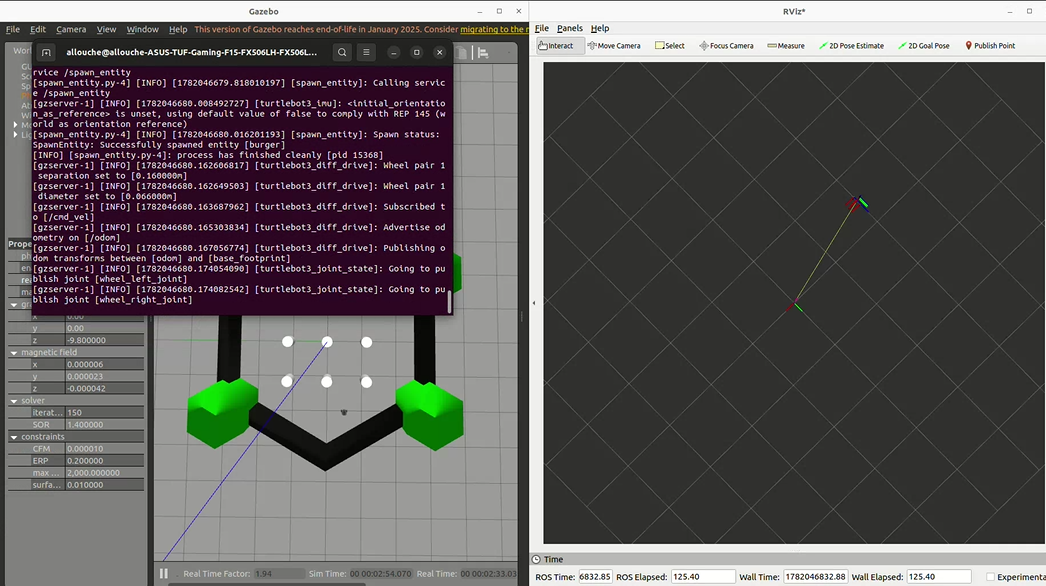
\includegraphics[width=\linewidth,height=4cm,keepaspectratio]{images/GazeboUltraSoundSimulationStartup.png}
		\caption*{\small (a) Startup.}
	\end{minipage}\hfill
	\begin{minipage}[b]{0.31\linewidth}
		\centering
		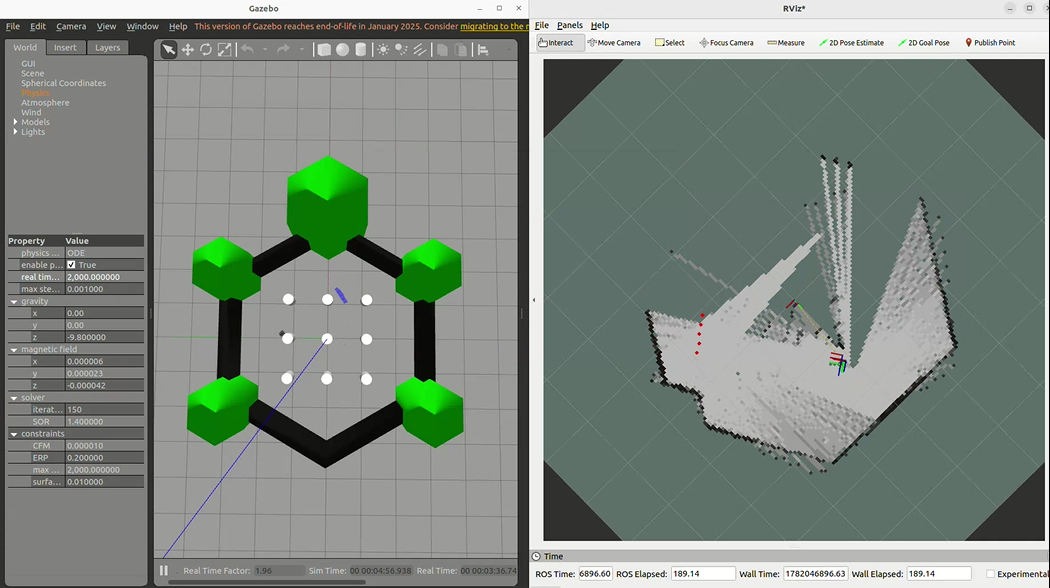
\includegraphics[width=\linewidth,height=4cm,keepaspectratio]{images/GazeboUltraSoundSimulationHalfProgress.png}
		\caption*{\small (b) Mid-exploration.}
	\end{minipage}\hfill
	\begin{minipage}[b]{0.31\linewidth}
		\centering
		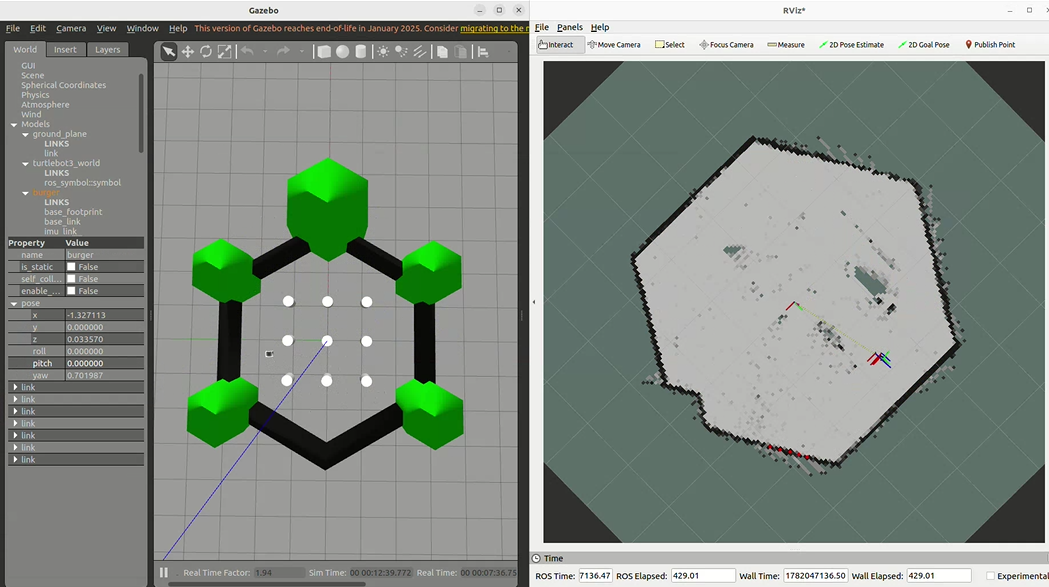
\includegraphics[width=\linewidth,height=4cm,keepaspectratio]{images/GazeboUltraSoundSimulationFinal.png}
		\caption*{\small (c) Final map.}
	\end{minipage}
	\caption{Gazebo simulation of ultrasonic occupancy-grid mapping (\texttt{ultrasonic\_slam\_simulation} branch). The robot autonomously explores a hexagonal arena using a AVANCER / EVITER / TOURNER state machine.}
	\label{fig:gazebo_ultrasound}
\end{figure}

The autonomous navigation relies on a three-state machine: \texttt{AVANCER} (forward at 0.07\,m/s), \texttt{EVITER} (obstacle avoidance at $<$0.85\,m), and \texttt{TOURNER} (rotation at $\pm$0.45\,rad/s). The Bayesian update runs at 20\,Hz (50\,ms timer), while the grid is published at 1\,Hz with Nav2-compatible QoS (\texttt{TRANSIENT\_LOCAL} + \texttt{RELIABLE}). As confirmed in Section~\ref{sec:slam_ultrasonic_vs_kinect}, this simulation demonstrated the limits of the slow ultrasonic sweep for real-time mapping, motivating the switch to the Kinect.

\section{Autonomous Navigation with Nav2}
\label{ch:navigation}

Autonomous navigation relies on the standard \textbf{Nav2} stack
(\texttt{navigation2.launch.py}, package \texttt{esibot\_navigation2}), loading the
static map, \texttt{esibot.yaml}, and orchestrating \gls{amcl} localization (500--2000 particles,
\texttt{likelihood\_field} + \texttt{DifferentialMotionModel}), costmaps, planner, controller,
velocity smoother and collision monitor. Local and global costmaps
\label{sec:nav_costmaps}
share 0.05\,m/cell resolution, 0.2\,m robot radius, 0.35\,m inflation radius.
\texttt{NavfnPlanner} (Dijkstra, 0.5\,m tolerance) feeds the \gls{dwb} local controller
(Table~\ref{tab:dwb_params}).

\begin{table}[H]
	\centering
	\caption{\gls{dwb} and \gls{amcl} kinematic bounds (excerpt from \texttt{esibot.yaml}).}
	\label{tab:dwb_params}
	\begin{tabularx}{\linewidth}{L{6cm} C{2.4cm} L{3.2cm}}
		\toprule
		\textbf{Parameter} & \textbf{Value} & \textbf{Unit} \\
		\midrule
		Min. / max. linear velocity (\gls{dwb}) & 0.2 / 0.3 & \unit{\metre\per\second} \\
		Max. angular velocity (\gls{dwb}) & 0.5 & \unit{\radian\per\second} \\
		Linear acceleration / deceleration & 3.0 / $-2.5$ & \unit{\metre\per\second\squared} \\
		Goal position tolerance (\texttt{FollowPath}) & 0.05 & \unit{\metre} \\
		Max. velocity (velocity smoother) & 0.5 / 2.5 & m/s / rad/s \\
		\bottomrule
	\end{tabularx}
\end{table}

The \gls{dwb} scoring criteria (\texttt{PathAlign} 32, \texttt{GoalDist} 24, \texttt{BaseObstacle} 0.02, \texttt{RotateToGoal} 32) favor path adherence. A \texttt{collision\_monitor} watches a stop disk (0.1\,m), a slowdown polygon, and an approach polygon (2\,s horizon). The default loaded map is a generic Nav2 sample; field validation with a real Kinect map is pending (Chapter~\ref{ch:resultats}).

\section{Autonomous Exploration}
\label{sec:slam_exploration}

The \texttt{working\_build} branch includes \texttt{src/m-explore-ros2} for frontier-based exploration (selects frontiers on \topic{/map}, sends goals to Nav2). Integration with the full bringup is pending: the submodule must be initialized, \topic{/map}/\topic{/tf} must be stable, and Nav2 must be active.
